\documentclass[%
  aps,
  pra,
  preprint,
  a4paper,
  amsmath,
  amssymb,
  floatfix,
  longbibliography,
  groupedaddress
]{revtex4-2}

% REVTeX already loads natbib and, with the class options above, amsmath/amssymb.
% Do not load cite, caption, or subcaption: they are incompatible with revtex4-2.
\usepackage{graphicx}
\usepackage{booktabs}
\usepackage{array}
\usepackage{longtable}
\usepackage{makecell}
\usepackage{siunitx}
\sisetup{inter-unit-product=\ensuremath{\cdot}}
\usepackage{etoolbox}
\setlength{\marginparwidth}{2cm}
\usepackage{todonotes}
\usepackage{url}

% REVTeX 4.2f does not recognize array.sty from 2024 and replaces both the
% column parser and longtable with older copies. Those copies cannot build
% p{} columns, so the parameter tables fail. Restore the current array and
% longtable definitions after the class has patched them.
\makeatletter
\let\CDR@mkpream\@mkpream
\let\CDR@classx\@classx
\let\CDR@array\@array
\let\CDR@tabular\@tabular
\let\CDR@tabarray\@tabarray
\let\CDR@@array\array
\let\CDR@endarray\endarray
\let\CDR@endtabular\endtabular
\let\CDR@arrayacol\@arrayacol
\let\CDR@tabacol\@tabacol
\let\CDR@insert@column\insert@column
\let\CDR@arraycr\@arraycr
\let\CDR@xarraycr\@xarraycr
\let\CDR@xargarraycr\@xargarraycr
\let\CDR@yargarraycr\@yargarraycr
\let\CDR@longtable\longtable
\let\CDR@endlongtable\endlongtable
\let\CDR@LT@start\LT@start
\let\CDR@LT@end\LT@end@hd@ft
\let\CDR@LT@array\LT@array
\AtBeginDocument{%
  \let\@mkpream\CDR@mkpream
  \let\@classx\CDR@classx
  \let\@array\CDR@array
  \let\@tabular\CDR@tabular
  \let\@tabarray\CDR@tabarray
  \let\array\CDR@@array
  \let\endarray\CDR@endarray
  \let\endtabular\CDR@endtabular
  \let\@arrayacol\CDR@arrayacol
  \let\@tabacol\CDR@tabacol
  \let\insert@column\CDR@insert@column
  \let\@arraycr\CDR@arraycr
  \let\@xarraycr\CDR@xarraycr
  \let\@xargarraycr\CDR@xargarraycr
  \let\@yargarraycr\CDR@yargarraycr
  \let\longtable\CDR@longtable
  \let\endlongtable\CDR@endlongtable
  \let\LT@start\CDR@LT@start
  \let\LT@end@hd@ft\CDR@LT@end
  \let\LT@array\CDR@LT@array
  % REVTeX removes \@makecol. longtable calls it when a table breaks
  % across pages; the page body is already boxed in \@cclv.
  \gdef\@makecol{\setbox\@outputbox\box\@cclv}%
}
\makeatother

\graphicspath{{img/}}
\hyphenation{pro-por-tional-ly}

% Empty subcaptions previously came from subcaption. This panel environment
% prints (a), (b), ... under each image without loading caption.sty.
\newcounter{panel}
\renewcommand{\thepanel}{\alph{panel}}
\AtBeginEnvironment{figure}{\setcounter{panel}{0}}
\newenvironment{panel}[2][c]{%
  \begin{minipage}[#1]{#2}%
    \centering
    \refstepcounter{panel}%
}{%
    \par\vspace{0.35em}{\footnotesize(\thepanel)}\par
  \end{minipage}%
}

\begin{document}

\title{Contribution from the EDM group to be included in the\\
SPRINT@NICA Conceptual Design Report\\
Search for the electric dipole moment of light nuclei at the NICA complex}

\author{V.~V. Fimushkin}
\author{A.~V. Butenko}
\author{E.~A. Butenko}
\author{N.~V. Dunin}
\author{K.~A. Ivshin}
\author{M.~V. Kulikov}
\author{S.~A. Kostromin}
\author{V.~P. Ladygin}
\author{V.~E. Laryonov}
\author{E.~M. Syresin}
\author{A.~N. Solovev}
\author{I.~S. Volkov}
\author{V.~A. Lebedev}
\author{E.~E. Donets}
\author{V.~V. Bleko}
\author{N.~M. Piskunov}
\author{A.~Ya. Silenko}
\author{O.~V. Teryaev}
\author{Yu.~N. Uzikov}
\author{A.~B. Borisov}
\author{E.~F. Dlin}
\affiliation{JINR}

\author{Yu.~N. Filatov}
\author{A.~N. Zelenski}
\author{S.~V. Vinogradov}
\author{S.~N. Zhabin}
\author{I.~S. Yudin}
\author{A.~A. Chernikova}
\author{E.~D. Tsyplakov}
\author{I.~V. Lilienberg}
\author{A.~I. Chernyshov}
\affiliation{MIPT}

\author{A.~E. Aksentiev}
\author{A.~S. Belov}
\author{Yu.~V. Senichev}
\author{S.~D. Kolokolchikov}
\author{A.~A. Melnikov}
\author{P. Palamarchuka}
\affiliation{INR RAS}

\author{N.~N. Nikolaev}
\affiliation{ITP}

\author{A.~M. Kondratenko}
\author{M.~A. Kondratenko}
\affiliation{STL Zaryad}

\author{V.~G. Baryshevsky}
\author{S.~V. Anischenko}
\author{A.~A. Gurinovich}
\affiliation{INP BSU}

\author{D.~K. Toporkov}
\affiliation{BINP SB RAS}

\maketitle

\tableofcontents

\clearpage

\section{Introduction}
\label{sec:introduction}

To be written. Long spin coherence time is a prerequisite for storage-ring
EDM experiments~\cite{JEDI:2016swi}.

\section{Lattice design principles for a storage-ring EDM search}
\label{sec:principles}

\subsection{Spin motion in electromagnetic fields}

The concept of an EDM measurement in a storage ring is based on the
Thomas--Bargmann--Michel--Telegdi (T-BMT)
equation~\cite{Bargmann:1959gz,Fukuyama:2013ioa}. In accordance with the
Ehrenfest theorem, it describes the classical spin motion of a charged particle
with a hypothetical EDM:
\begin{equation}
\begin{aligned}
  \frac{d\vec{S}}{dt} &= \left(\vec{\Omega}_{mdm} + \vec{\Omega}_{edm}\right)\times\vec{S},\\
  \vec{\Omega}_{mdm} &= -\frac{e}{m\gamma}\left\{(\gamma G+1)\vec{B}_{\perp}
     + (1+G)\vec{B}_{\parallel}
     - \left(\gamma G+\frac{\gamma}{\gamma+1}\right)\frac{\vec{\beta}\times\vec{E}}{c}\right\},\\
  \vec{\Omega}_{edm} &= -\frac{e\eta}{2m}\left(\vec{\beta}\times\vec{B}+\frac{\vec{E}}{c}\right),
  \qquad G = \frac{g-2}{2},
\end{aligned}
\label{eq:tbmt}
\end{equation}
where $\gamma$ is the Lorentz factor, $\vec{\beta}$ is the relative velocity,
$c$ is the speed of light, $e$ and $m$ are the particle charge and mass, $G$ is
the magnetic anomaly, $g$ is the gyromagnetic ratio, $\Omega_{mdm}$ and
$\Omega_{edm}$ are the spin precession frequencies due to the magnetic and
electric dipole moments, $\eta$ is a dimensionless coefficient defined by
$d = \eta e\hbar/4mc$, and $\vec{B}=\{B_\perp, B_\parallel\}$ and
$\vec{E}=\{E_\perp, E_\parallel\}$ are the magnetic and electric fields. Since
no elements with a longitudinal magnetic field are used, we set
$B_\parallel = 0$; the longitudinal electric field is neglected as well,
$E_\parallel = 0$, because its contribution is small.

The lattice must provide conditions under which the EDM signal continuously
accumulates while the beam circulates in the ring. To this end, the spin and
the longitudinal momentum must remain aligned, $\vec{S}\uparrow\uparrow\vec{p}$,
with a precision that determines the attainable sensitivity of the EDM
measurement. Depending on the precision and the method of its realization,
this condition is referred to as the frozen spin or, more generally, the
quasi-frozen spin condition~\cite{Senichev:2016rez}.

\subsection{Frozen spin concept}

The idea of searching for the proton and deuteron EDMs with polarized beams in
a storage ring is based on the frozen spin (FS) method originally proposed at
the Brookhaven National Laboratory~\cite{Farley:2004hp,srEDM:2008}. An FS
lattice consists of deflectors combining electric and magnetic fields in one
element, in which the spin of the reference particle always stays along the
momentum.

The frozen spin method relies on the fact that at a specific, so-called
``magic'' energy the spin precesses in the external fields with the same
frequency as the particle momentum,
$\Omega^{p}_{E,B} = \frac{eE}{m\gamma\beta c} + \frac{eB}{m\gamma}$.
Subtracting this frequency from $\vec{\Omega}_{mdm}$ gives the spin precession
frequency relative to the momentum:
\begin{equation}
  \vec{\Omega}^{p}_{mdm} = \vec{\omega}^{p}_{E} + \vec{\omega}^{p}_{B},
  \label{eq:omega_p}
\end{equation}
where
$\vec{\omega}^{p}_{E} = \frac{e}{m}\left(G-\frac{1}{\gamma^2-1}\right)\frac{\vec{E}\times\vec{\beta}}{c}$
and $\vec{\omega}^{p}_{B} = \frac{e}{m}G\,\vec{B}_{\perp}$ are the
contributions of the electric and magnetic fields. In a purely electrostatic
ring ($\vec{B}=0$) the frozen spin condition $\vec{\omega}^{p}_{E} = 0$ is
satisfied at the magic energy
\begin{equation}
  G - \frac{1}{\gamma_{mag}^2-1} = 0 .
  \label{eq:magic}
\end{equation}
In a ring with both magnetic and electric elements, the frozen spin condition
$\vec{\Omega}^{p}_{mdm}=0$ is achieved by balancing the radial electric field
$E_r$ against the vertical guiding magnetic field $B_v$~\cite{srEDM:2008}:
\begin{equation}
  E_r = \frac{G B_v c\beta\gamma^2}{1-G\beta^2\gamma^2} \approx G B_v c\beta\gamma^2 .
  \label{eq:fs_hybrid}
\end{equation}
A hybrid ring is required for deuterons because their magnetic anomaly is
negative, $G = -0.143$, and condition~\eqref{eq:magic} cannot be satisfied.

It is convenient to introduce the spin tune, i.e., the number of spin
precessions per revolution. In an electrostatic ring the spin tune relative
to the momentum is $\nu_s^E = \omega^p_E/\Omega^p_E$:
\begin{equation}
  \nu_s^E = \left(G-\frac{1}{\gamma^2-1}\right)\gamma\beta^2 ,
  \label{eq:nu_e}
\end{equation}
and in a magnetic field, $\nu_s^B = \omega^p_B/\Omega^p_B$:
\begin{equation}
  \nu_s^B = \gamma G .
  \label{eq:nu_b}
\end{equation}
Thus, the same concept applies to protons and deuterons, but it is realized
with different types of deflectors.

\subsection{Quasi-frozen spin concept}

In the NICA ring, an implementation of the FS concept would require a
complete rebuild of the optics. Suppose instead that the spin oscillates in
the horizontal plane around the frozen spin direction with a small amplitude,
$\Phi_s^2 \ll 1$. This can be done with special electric-field elements in the
straight sections, which bring the spin back along the momentum after it has
deviated in the magnetic arc. The EDM signal growth is then reduced by the
factor $J_0(\Phi_s)\approx 1-\Phi_s^2/4$. The deuteron magnetic anomaly
$G=-0.143$ is small, and the spin oscillates around the momentum within half of
the spin phase advance in the magnetic arc,
$\Phi_s = \pi\gamma G/2 \approx 0.25$. Therefore, at the optimal parameters of
the EDM measurement, $\gamma = 1.12$, the effective EDM signal is reduced by
only a few percent.

This gives the essence of the quasi-frozen spin
concept~\cite{Senichev:2016rez}: the spin is not frozen relative to the
momentum but continuously oscillates around an average fixed direction that
coincides with the momentum direction. The question to be answered next is how
to implement a variable MDM spin precession in the storage ring, which is
needed for its zero average over the statistics, while providing a sufficient
growth of the EDM signal.

Two QFS options exist. In the first one, the magnetic and electric fields are
completely separated in space: the magnetic field acts in the arcs and the
electric field acts in the straight sections, which are realized as
negative-curvature ``reverse'' electrostatic arcs. This option inherits the
drawback of cylindrical electrodes, namely, a whole set of high-order field
nonlinearities. In the second option, a small magnetic field of about
\SI{100}{mT} is added to the spin-aligning E+B elements; it compensates the
Lorentz force of the electric field and makes the elements straight. Such an
E+B element is a Wien filter. The second option is the most appropriate one
for rings not designed specifically for the EDM search, in particular for the NICA ring
with bypass sections, whereas for the Nuclotron, where the free
space is limited, the first option is the baseline.

\subsection{Parameters of the Wien filters}
\label{sec:wien}

In a magnetic arc the momentum is rotated by the angle $\Phi^B_{arc}$, and the
spin simultaneously rotates in the horizontal plane relative to the momentum
by the angle
\begin{equation}
  \Phi_s^{arc} = \gamma G\,\Phi^B_{arc} .
  \label{eq:phi_arc}
\end{equation}
In the E+B elements of the straight section, the spin rotation relative to the
momentum has two components. In the electric field it is opposite to the
momentum rotation,
\begin{equation}
  \Phi_s^{E} = -\left(\gamma G+\frac{\gamma}{\gamma+1}\right)\beta^2\,\Phi^{E}_{ss},
  \label{eq:phi_e}
\end{equation}
where $\Phi^E_{ss}$ is the momentum rotation angle in the electric field. In
the magnetic field the spin rotates in the same direction as the momentum,
$\Phi_s^B = (\gamma G+1)\,\Phi^B_{ss}$, where $\Phi^B_{ss}$ is the momentum
rotation angle in the magnetic field. Since the Lorentz force vanishes, the
two momentum rotation angles are equal, $\Phi^E_{ss} = \Phi^B_{ss}$, and both
spin rotations can be expressed through one of them, e.g., through
$\Phi^B_{ss} = \frac{eB_{ss}}{m\gamma v}L_{ss}$, where $B_{ss}$ and $L_{ss}$
are the magnetic field and the length of the straight element. The QFS
condition requires that the net spin rotation in the E+B elements compensate
the spin rotation in the arc, $\Phi_s^B + \Phi_s^E = \Phi_s^{arc}$. For an arc
bending the beam by $\Phi^B_{arc}=\pi$ this gives
\begin{equation}
  (\gamma G+1)\,\Phi^B_{ss} - \left(\gamma G+\frac{\gamma}{\gamma+1}\right)\beta^2\,\Phi^E_{ss} = \pi\gamma G .
  \label{eq:qfs}
\end{equation}
Simple transformations yield the parameters of the E+B elements:
\begin{equation}
  L_\Sigma E_{ss} = \frac{G}{G+1}\,\frac{mc^2}{e}\,\pi\beta^2\gamma^3,
  \qquad
  B_{ss} = -\frac{E_{ss}}{c\beta},
  \label{eq:wien}
\end{equation}
where $L_\Sigma$ is the total length of the straight elements in one straight
section. For a realistic electric field of \SI{100}{kV/cm}, the corresponding
magnetic field is below \SI{96}{mT}. This simplifies the technical design: a
permanent magnet or an air-core coil can be used.

The material of this section has been reported
in~\cite{Senichev:2016rez,Senichev:2024qtr,Melnikov:2025gdj,Melnikov:2025ytd,Senichev:2025jqf}.

\section{NICA bypasses}
\label{sec:nica-bypass}

To be written.

\section{Modernized Nuclotron}
\label{sec:nuclotron}

\subsection{Present Nuclotron lattice}

Figure~\ref{fig:nica_complex} shows the NICA accelerator complex, which
comprises the Booster, the Nuclotron and the Collider. The Booster and the
Nuclotron serve as the injector of heavy ions, polarized protons and
deuterons into the collider. The Nuclotron lattice was originally designed to
be as close to circular as possible and has eight superperiods.
Figure~\ref{fig:nuclotron_twiss} shows the Twiss functions of one superperiod,
which consists of a bending arc of three FODO cells, each with four bending
magnets with a maximum field of \SI{1.8}{T}, and a straight section of one FODO
cell. The Nuclotron circumference is \SI{251}{m}.

\begin{figure}[htbp]
  \centering
  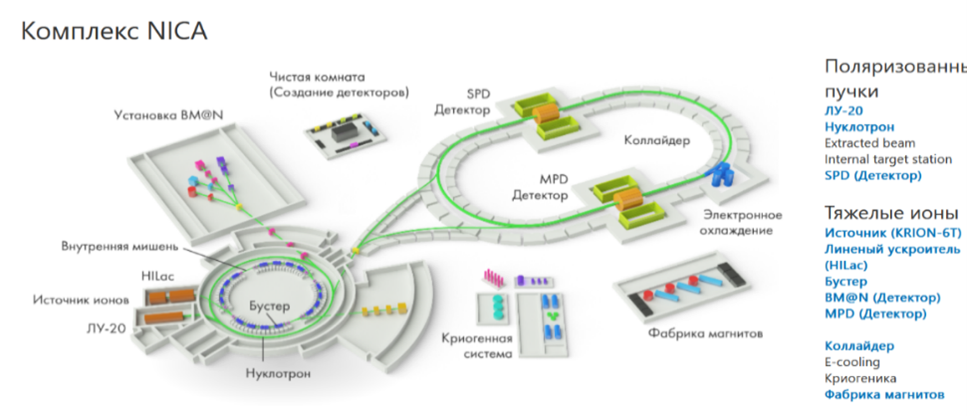
\includegraphics[width=0.7\textwidth]{nica_complex}
  \caption{NICA accelerator complex.}
  \label{fig:nica_complex}
\end{figure}

\begin{figure}[htbp]
  \centering
  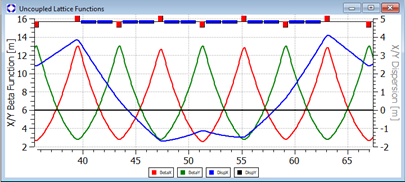
\includegraphics[width=0.7\textwidth]{nuclotron_twiss}
  \caption{Twiss functions of one Nuclotron superperiod.}
  \label{fig:nuclotron_twiss}
\end{figure}

The main drawback of the Nuclotron, both as a collider injector and as a
stand-alone ring, is the limited length of the drift spaces in which the
equipment for these two functions must be installed. All modernization options below
are assessed with respect to this limitation.

\subsection{Modernization options}

Two modernization options of the Nuclotron have been studied.

The first option, Nuclotron~2.1, is a lattice that preserves all properties of
the existing accelerator and allows deuteron EDM experiments with electric
deflectors or Wien filters installed in the ring. Either device keeps the spin
of the polarized beam along its direction of motion around the ring. Within the
eight-superperiod lattice, $N_{super} = 8$, this requires implementing the
frozen (or quasi-frozen) spin concept by lengthening the straight sections
between the arcs, ensuring zero dispersion in the straight sections, and, if
possible, keeping the ring circumference so that the equipment fits into the
existing tunnel. An axion search could also be included in this framework,
although the treatment of the systematic errors of such an experiment is not
yet fully understood. In the Nuclotron~2.1 option, all key collider
parameters, such as the transition energy and the electron cooler parameters,
remain unchanged. This creates a serious problem at the interface between the
collider and the Nuclotron: crossing the transition energy with a cooled beam
leads to irreversible beam degradation and a lower final luminosity.

The Nuclotron~2.2 option introduces modifications that ensure compatibility
with the collider. The injection energy of polarized protons into the collider
remains at 2--\SI{3}{GeV}. To eliminate the effect of transition crossing after
electron cooling, the transition energy of the collider is to be raised above
its maximum operating energy. In addition, a lower maximum energy of heavy ions
and polarized particles in Nuclotron~2.2 is considered. This frees space in the
ring for Wien filters and extends the capabilities of the Nuclotron for EDM and
axion experiments. A lower Nuclotron energy does not degrade the complex as a
whole, since the collider can take over some functions of the Nuclotron and
provide proton and heavy-ion beams over the entire Nuclotron energy range.

\subsection{Nuclotron 2.1: quasi-frozen spin for deuterons}

Adapting the Nuclotron lattice to the measurement of the deuteron EDM involves
three problems: lengthening the straight sections, suppressing the dispersion
in the straight sections, and keeping the spin direction along the momentum
around the ring.

The first problem is solved by raising the maximum field of the bending
magnets to \SI{1.8}{T} and by merging the two adjacent magnets between the
quadrupoles into one magnet. At the same time, the dispersion is suppressed by
choosing the horizontal phase advance in the arcs. One superperiod of the
modernized Nuclotron~2.1 is shown in Fig.~\ref{fig:nuclotron21}. The main
parameters of Nuclotron~2.1 are: circumference \SI{251}{m}; betatron tunes
$Q_x = 9.78548$, $Q_y = 10.6839$; momentum compaction factor 0.0134394; slip
factor $-0.0222388$; natural chromaticity $-16.0394$ (horizontal) and
$-17.8984$ (vertical). In the figure, D denotes a defocusing quadrupole, F a
focusing quadrupole, B a dipole magnet and ED an electrostatic deflector. The
parameters of all options are summarized in Table~\ref{tab:nuclotron}.

\begin{figure}[htbp]
  \centering
  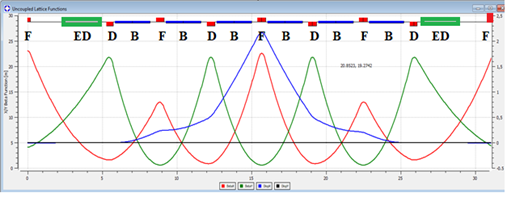
\includegraphics[width=0.8\textwidth]{nuclotron21_twiss}
  \caption{Twiss functions of one superperiod of the modernized Nuclotron~2.1
    with two electrostatic deflectors.}
  \label{fig:nuclotron21}
\end{figure}

With the bending field raised to \SI{1.8}{T}, the length of the straight
section in each superperiod increases from 7.3 to \SI{10.5}{m}. The third
problem, keeping the spin direction relative to the momentum as required for
the detection of the deuteron EDM signal, is solved with negative-curvature
electrostatic deflectors in each superperiod (Fig.~\ref{fig:nuclotron_ed}).

In the quasi-frozen spin concept, the magnetic and electric fields act in
different elements. The spin direction therefore oscillates relative to the
direction of motion, since the spin rotates in opposite directions in the
magnetic and electrostatic bending elements. The deuteron magnetic anomaly is
small, $G = -0.143$. The spin oscillates around the momentum in each magnetic
arc within half of the spin phase advance,
$\Phi_s = \frac{1}{2N}\,2\pi\gamma G$, and each time it is turned back by
$-\Phi_s$ in the electrostatic deflector; here $N$ is the arc superperiodicity.
This keeps the average spin direction along the momentum around the whole ring,
in accordance with the quasi-frozen spin concept~\cite{Senichev:2020qfs}.

For the Nuclotron, $N = 8$. Owing to the small value of $\Phi_s$, the effective
EDM signal is reduced only by the factor
\begin{equation}
  J_0(\Phi_s) \approx 1 - \frac{\Phi_s^2}{4},
\end{equation}
i.e., by a few percent at most.

To determine the parameters of the electrostatic deflectors in the
quasi-frozen spin mode for deuterons, consider the lattice as consisting of
two different parts (Fig.~\ref{fig:nuclotron_ed}). The magnetic arcs bend the
beam by $\Phi^B = 2\pi/N + 2\alpha$ each and rotate the spin in the horizontal
plane relative to the momentum by $\Phi^B_s = \nu^B_s\Phi^B$. The electrostatic
arcs with negative-curvature deflectors bend the beam by $\Phi^E = -2\alpha$
each and rotate the spin relative to the momentum in the opposite direction by
$\Phi^E_s = \nu^E_s\Phi^E$. The quasi-frozen spin condition requires
$\Phi^E_s = -\Phi^B_s$. Since in an electrostatic deflector the spin rotates
relative to the momentum many times faster than in a magnetic field, the two
types of arcs are related by
\begin{equation}
  \nu_s^B\left(\frac{2\pi}{N}+2\alpha\right) = \nu_s^E\, 2\alpha,
  \qquad
  \alpha = \frac{1}{\nu_s^E/\nu_s^B-1}\,\frac{\pi}{N} = -\gamma^2\frac{G}{G+1}\,\frac{\pi}{N},
  \label{eq:nuclotron_alpha}
\end{equation}
where $\nu_s^E$ and $\nu_s^B$ are given by Eqs.~\eqref{eq:nu_e}
and~\eqref{eq:nu_b}. For given bending magnets and a deflector field
$E_{ED} = \SI{130}{kV/cm}$, one obtains $\nu_s^E/\nu_s^B$, the parameter
$\alpha$ and the radius of curvature of the deflector $R_{ED} = \kappa/E_{ED}$,
where $\kappa = p_0\beta c/e$ is the electric rigidity and
$p_0 = \gamma m\beta c$, so that
$R_{ED} = \frac{mc^2}{e}\frac{\gamma\beta^2}{E_{ED}}$. The deflector length is
then
$L_{ED} = 2\alpha R_{ED} = -2\frac{\gamma^2 G}{G+1}\frac{\pi}{N}R_{ED}$.
Figure~\ref{fig:nuclotron_ed} shows how the electrostatic deflectors are
inserted to realize the quasi-frozen spin lattice of the Nuclotron. At the
optimal polarimeter energy $W = \SI{270}{MeV}$~\cite{Kurilkin:2010ym},
$\alpha = 0.026\pi$ and the required length of the electrostatic channel is
\SI{7.3}{m}. The EDM signal relative to the frozen spin case,
$S^{QFS}_{EDM}/S^{FS}_{EDM} = 1-\alpha^2/4 \approx 0.998$, is reduced by only
0.2\%.

The electrostatic arc with negative curvature leaves room for the necessary
equipment in the straight section between two magnetic arcs; when the
electrostatic deflectors are switched off, the beam passes straight through
this section.

\begin{figure}[htbp]
  \centering
  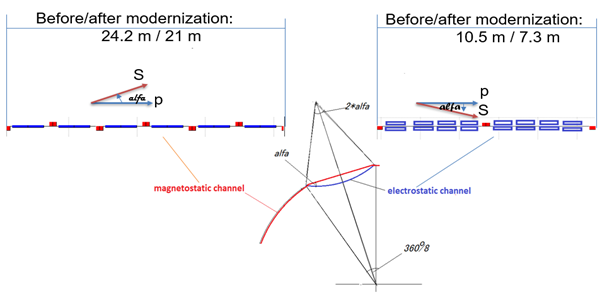
\includegraphics[width=0.8\textwidth]{nuclotron_ed_insert}
  \caption{Electrostatic insertion compensating the spin rotation in the
    magnetic arc.}
  \label{fig:nuclotron_ed}
\end{figure}

A lattice with twice the number of superperiods, 16, was also considered.
By splitting the double bending magnets into individual magnets, the number of
FODO cells per superperiod is doubled, and with a \ang{60} phase advance per
FODO cell the dispersion is suppressed in every second straight section. In
this version $\alpha = 0.013\pi$, and the EDM signal relative to the frozen spin
case is $1-\alpha^2/4 \approx 0.9996$, i.e., reduced by only 0.04\%, which makes
this lattice practically equivalent to the frozen spin one. This lattice can
also be used for the proton EDM, since the spin rotation angle of protons in
the magnetic arcs is only about \ang{30}.

\subsection{Nuclotron 2.2: quasi-frozen spin with Wien filters for deuterons}

In the Nuclotron~2.2 lattice, a small vertical magnetic field of about
\SI{100}{mT} is added to compensate the Lorentz force of the electric field,
so that the electrostatic deflectors become straight. With the magnetic field
added, the E+B element is a Wien filter. The ring then consists of arcs
connected by straight sections with Wien filters, in which crossed electric
and magnetic fields keep the particles on a straight path (zero Lorentz force)
and compensate the spin rotation accumulated in the magnetic arcs. The total
length of the Wien filters is determined by the beam parameters and by the
required compensation of the spin rotation in the arcs, whereas their number
is chosen for convenient placement around the ring.

With $N$ magnetic arcs in total, each arc bends the particles by
$\Phi^B_{arc} = 2\pi/N$ and rotates the spin in the horizontal plane relative
to the momentum by $\Phi^{arc}_s = \gamma G\,\Phi^B_{arc}$. The Wien filters
rotate the spin relative to the momentum in the opposite direction. In the
electric field $E_{wf}$ the spin rotation angle is
\begin{equation}
  \Phi^E_{swf} = -\left(\gamma G+\frac{\gamma}{\gamma+1}\right)\beta^2\,\Phi^E_{wf},
\end{equation}
where $\Phi^E_{wf} = \frac{eE_{wf}}{m_0c^2\gamma\beta^2}L_{wf}$ is the momentum
rotation angle in the electric field of the Wien filter, and in the magnetic
field $B_{wf}$ it is
\begin{equation}
  \Phi^B_{swf} = (\gamma G+1)\,\Phi^B_{wf},
\end{equation}
where $\Phi^B_{wf} = \frac{eB_{wf}}{m_0c\gamma\beta}L_{wf}$ is the momentum
rotation angle in the magnetic field of a Wien filter of length $L_{wf}$.

Since the Lorentz force in the Wien filter vanishes, the angles must be equal,
$\Phi^E_{wf} = \Phi^B_{wf}$, and they can be expressed through the electric
field $E_{wf}$ and the length $L_{wf}$ of the filters installed in all $N$
straight sections. In the frozen spin option, the total spin precession
frequency relative to the momentum in the combined E+B bending element is
zero. The quasi-frozen spin option instead requires the total spin rotation
angle per turn in the E and B fields to vanish. The QFS condition therefore
reads
\begin{equation}
  (\gamma G+1)\,\Phi^B_{wf} - \left(\gamma G+\frac{\gamma}{\gamma+1}\right)\beta^2\,\Phi^E_{wf} = \gamma G\,\frac{2\pi}{N},
\end{equation}
which gives the parameters of one Wien filter:
\begin{equation}
  L_{wf}E_{wf} = \frac{2\pi}{N}\,\frac{G}{G+1}\,\frac{m_0c^2}{e}\,\beta^2\gamma^3,
  \qquad
  B_{wf} = -\frac{E_{wf}}{c\beta},
  \label{eq:nuclotron_wf}
\end{equation}
where $L_{wf}$ is the length of one Wien filter. The total length of all Wien
filters,
$L^\Sigma_{wf}E_{wf} = 2\pi\frac{G}{G+1}\frac{m_0c^2}{e}\beta^2\gamma^3$,
depends only on the particle species and energy.

Equations~\eqref{eq:nuclotron_alpha} and~\eqref{eq:nuclotron_wf}, derived for
electrostatic deflectors and for Wien filters, show that the type of the
compensating element does not matter. With the magnetic arc unchanged, the
Wien filters are shorter by the total length of the kickers, since a Wien filter
combines the functions of an electrostatic deflector and a kicker in one
element.

Figure~\ref{fig:nuclotron221} shows the Twiss functions of one superperiod of
the first version of the modernized lattice, Nuclotron~2.2.1. Two Wien filters
installed in the central straight sections of the superperiod restore the spin
direction after each magnetic half-arc. The spin deviation angle from the
momentum, $\alpha = \gamma G\,2\pi/N$, characterizes how much the quasi-frozen
spin lattice differs from the frozen spin one. In this lattice, the number of
arcs that determine the spin deviation equals the number of superperiods,
$N = 8$.

\begin{figure}[htbp]
  \centering
  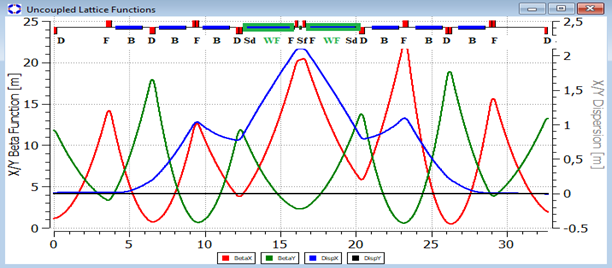
\includegraphics[width=0.8\textwidth]{nuclotron221_twiss}
  \caption{Twiss functions of one superperiod of the modernized
    Nuclotron~2.2.1 with two Wien filters.}
  \label{fig:nuclotron221}
\end{figure}

For a maximum electric field of \SI{130}{kV/cm}, the magnetic field is below
\SI{80}{mT}. Such a low magnetic field simplifies the Wien filter design: a
permanent magnet or an air-core coil can be used. For these fields and a
deuteron energy of \SI{270}{MeV}, the total length of the Wien filters in all
straight sections is about \SI{52}{m}, and the length of one Wien filter is
\SI{3.25}{m}. At \SI{270}{MeV} (\SI{135}{MeV} per nucleon), the maximum spin
deviation is $\alpha\sim\pm\ang{3}$ over one arc, which is a good
approximation to a regular frozen spin lattice.

In the next version, Nuclotron~2.2.2, the Wien filters are distributed over
four straight sections of the superperiod (Fig.~\ref{fig:nuclotron222}). Each
arc of the superperiod is thus split into two arcs, and with respect to the
bending magnets the lattice has the superperiodicity $N = 16$, while the overall
superperiodicity of the lattice with all elements remains 8. This solves two
problems. First, the ring becomes a 16-sided polygon, i.e., closer to a circle,
and fits the existing tunnel better. Second, with a bending magnet length of
\SI{1.77}{m} and a Wien filter length of \SI{1.65}{m}, the spin deviation is
$\alpha\sim\pm\ang{1.5}$, half that of version~2.2.1. This brings the
properties of the quasi-frozen spin lattice much closer to those of the frozen
spin lattice.

\begin{figure}[htbp]
  \centering
  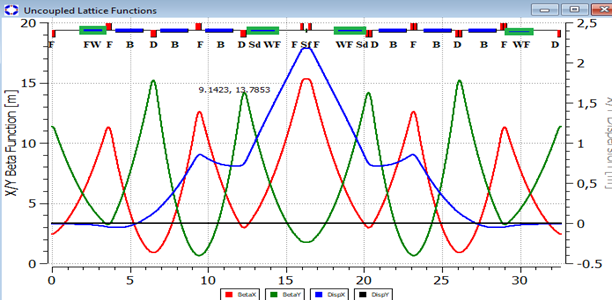
\includegraphics[width=0.8\textwidth]{nuclotron222_twiss}
  \caption{Twiss functions of one superperiod of the modernized
    Nuclotron~2.2.2 with four Wien filters.}
  \label{fig:nuclotron222}
\end{figure}

To increase the energy, the modification Nuclotron~2.2.3 with fewer empty
drift spaces and longer magnets was considered (Fig.~\ref{fig:nuclotron223}).
In this lattice, the maximum energy is \SI{3.5}{GeV} per nucleon for deuterons
and \SI{7.8}{GeV} for protons, which is much closer to the present Nuclotron.

\begin{figure}[htbp]
  \centering
  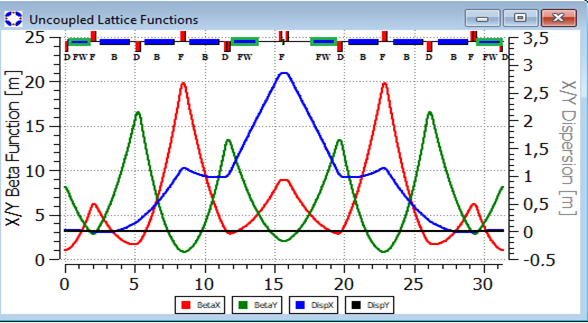
\includegraphics[width=0.75\textwidth]{nuclotron223_twiss}
  \caption{Twiss functions of one superperiod of the modernized
    Nuclotron~2.2.3 with four Wien filters.}
  \label{fig:nuclotron223}
\end{figure}

\begin{table}[htbp]
  \centering
  \caption{Main parameters of the Nuclotron modifications.}
  \label{tab:nuclotron}
  \footnotesize
  \setlength{\tabcolsep}{2.5pt}
  \begin{tabular}{lcccccccc}
    \toprule
    \makecell[l]{Nuclotron\\lattice} & \makecell{Magnet\\length, m} & \makecell{Number of\\magnets}
      & \makecell{Total magnet\\length, m} & \makecell{$B_{max}$,\\T}
      & \makecell{$B_{max}R$,\\T$\cdot$m} & \makecell{$W_d^{max}$,\\GeV}
      & \makecell{$W_d^{max}$,\\GeV/u} & \makecell{$W_p^{max}$,\\GeV} \\
    \midrule
    Present & 1.44 & 96 & 138.24 & 1.8 & 39.6  & 10.14 & 5.07 & 10.97 \\
    2.1     & 2.35 & 48 & 112.77 & 1.8 & 32.2  & 8     & 4    & 8.79 \\
    2.2.1   & 1.78 & 48 & 85.3   & 1.8 & 24.4  & 5.7   & 2.85 & 6.47 \\
    2.2.2   & 1.78 & 48 & 85.44  & 1.8 & 24.5  & 5.7   & 2.85 & 6.47 \\
    2.2.3   & 2.10 & 48 & 101    & 1.8 & 28.93 & 7.0   & 3.5  & 7.8 \\
    \bottomrule
  \end{tabular}
\end{table}

\subsection{Nuclotron 2.2.2: quasi-frozen spin with Wien filters for protons}

With a magnetic superperiodicity of 16, the lattice can also be used for
protons at a reduced energy. The energy is then limited mainly by the free
space for the Wien filters, which is \SI{52}{m} in this lattice. The maximum
proton energy follows from Eq.~\eqref{eq:nuclotron_wf}:
\begin{equation}
  \gamma(\gamma^2-1) = L_{wf}\,\frac{eE_{wf}}{mc^2}\,\frac{N}{2\pi}\,\frac{G_p+1}{G_p},
\end{equation}
where $L_{wf}N = \SI{52}{m}$ and $G_p = 1.793$ is the proton magnetic anomaly.
Solving for $\gamma$ gives $\gamma = 1.08047$, i.e., $W_p\approx\SI{80}{MeV}$.
At this energy, the spin deviation in a magnetic arc is determined by
$\gamma G_p = 1.93711$, and the spin deviation angle is
$\alpha = \pm\frac{1}{2}\frac{\gamma G_p}{16}$, which amounts to
$\alpha = \ang{3.5}$.\todo[inline]{Check: with the factor $2\pi$ of
Eq.~\eqref{eq:nuclotron_wf}, $\alpha=\pm\frac12\gamma G_p\frac{2\pi}{16}\approx\ang{22}$.}
The same lattice as for deuterons can be used for protons, but at a lower
energy and with the Wien filters rotated by \ang{180}, since the magnetic
anomalies of the two particles have opposite signs. At a proton energy of
\SI{80}{MeV} the lattice thus behaves practically as a frozen spin lattice.
Figure~\ref{fig:pc_ay} shows the p--C analyzing power in terms of the
``average analyzing power'' taken from Ref.~\cite{Mcnaughton:1985wyt}.

\begin{figure}[htbp]
  \centering
  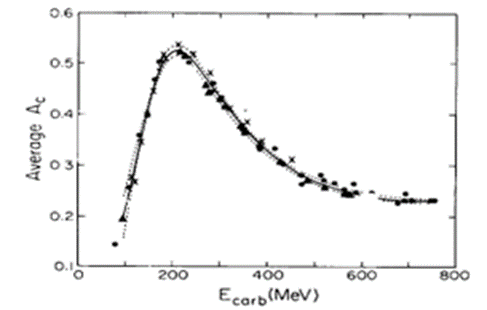
\includegraphics[width=0.6\textwidth]{pc_analyzing_power}
  \caption{Average p--C analyzing power $\overline{A_c}$ for
    $\theta_{lab} = \ang{5}$--\ang{20} at discrete energies (points) and its
    continuous energy dependence (solid line). The data are from SIN
    ($\triangle$), TRIUMF ($\times$) and LAMPF ($\bullet$)~\cite{Mcnaughton:1985wyt}.}
  \label{fig:pc_ay}
\end{figure}

Figure~\ref{fig:pc_ay} shows that the analyzing power near \SI{100}{MeV} is
about 0.2, i.e., 0.35 of its maximum value $A_c = 0.53$ at \SI{230}{MeV}. This
makes proton EDM studies at this energy in the Nuclotron~2.2.2 lattice
feasible in parallel with full-scale deuteron measurements.

Galactic axions can be searched for with the same equipment as the EDM.
Varying the spin precession frequency at a fixed beam energy turns the booster
with Wien filters into a broadband antenna that searches for axions through a
resonant full or partial spin flip in the oscillating pseudomagnetic field of
the axion halo of our Galaxy~\cite{Nikolaev:2022wyi}. The growth of the
horizontal polarization induced by axions is extracted by a Fourier analysis of
the oscillating vertical asymmetry in the internal
polarimeter~\cite{JEDI:2015vwa}.

\subsection{Maximum energy of heavy ions and protons in Nuclotron 2.2.2}

The calculations show that deuteron and proton EDM experiments in the
Nuclotron~2.2.2 lattice require free space for Wien filters with a total length
of \SI{52}{m}. With the tunnel circumference fixed at \SI{251}{m}, this is
possible either by raising the field of the bending magnets, which is already
set to \SI{1.8}{T}, or by reducing their total length. Assuming that the
bending field does not exceed \SI{1.8}{T}, the second option was chosen, which
inevitably lowers the maximum particle energy in the Nuclotron.

\subsection{Features of the modernized Nuclotron lattice}

The lattice of the modernized Nuclotron was designed with several goals.
First, the superperiod has a drift without bending magnets in its central
cell, where the dispersion function reaches its maximum and the orbit
curvature is zero ($\rho\to\infty$). This makes it possible to raise the
transition energy, since the momentum compaction factor is
\begin{equation}
  \alpha = \frac{1}{C}\oint\frac{D(s)}{\rho(s)}\,ds .
\end{equation}
Second, the number of superperiods $s = 8$ is only slightly larger than the
horizontal betatron tune $\nu_x$, which makes the momentum compaction factor
easy to adjust, as in the resonant lattices with a low or negative momentum
compaction factor~\cite{Senichev:1997kn,Ishi:1998tj,Papaphilippou:2010zz,Senichev:2008zza,Toelle:2007zz}:
\begin{equation}
  \alpha = \frac{\nu_x^3}{R}\sum_{k=0}^{\infty}\frac{a_k^2}{\nu_x^2-(ks)^2},
\end{equation}
where $a_k$ are the harmonics of the dispersion-generating perturbation.
Third, the central drift simplifies the placement of the three sextupole
families needed to control the betatron and spin chromaticities, whereas the
side drifts are convenient for the Wien filters. Finally, the maximum of the
dispersion at the center of the superperiod coincides with the minimum of the
horizontal beta function $\beta_x$.

\subsection{Summary}

If the Nuclotron is used as the booster of the collider, its final energy can
be lowered to 2--\SI{3}{GeV} without a significant degradation of the NICA
complex, because all physics experiments with polarized beams are transferred
to the collider. This choice has a further advantage: it shortens the total
length of the bending magnets, e.g., by reducing each double bending magnet of
the Nuclotron to one section, and frees about \SI{70}{m} of the orbit for
additional equipment, in particular for polarization-preserving solenoids. It
also provides room for EDM and axion search equipment directly in the
Nuclotron.

The material of this section has been reported
in~\cite{Senichev:2023vtx,Senichev:2024fey,Senichev:2025ude,Senichev:2026xca,Kolokolchikov:2025sew,Senichev:2025jqf}.

\section{Specialized frozen spin rings at JINR}
\label{sec:specialized-ring}

This section presents two specialized frozen spin lattices designed
exclusively for the search for the electric dipole moments of the proton and
the deuteron: an all-electrostatic ring for protons and a ring with combined
E+B deflectors for deuterons.

\subsection{Frozen spin option for the proton beam}

The frozen spin lattice for a proton beam is the simplest one in terms of
parameter choice and is uniquely defined. It consists of electrostatic
deflectors whose total length $L_{total}$ is determined by the beam energy and
the maximum permissible electrostatic field strength:
\begin{equation}
  L_{total} = 2\pi\,\frac{mc^2}{eE}\,\gamma\beta^2 .
  \label{eq:pring_length}
\end{equation}
For an energy of \SI{233}{MeV} and a maximum field of $E = \SI{120}{kV/cm}$,
the total length of all electrostatic deflectors is $L_{total} = \SI{219.55}{m}$.

With 50 deflectors placed around the ring, the length of a single deflector is
$L_{def} = \SI{4.39}{m}$. The 50 deflectors are divided into five groups, each
consisting of five FODO cells and containing ten deflectors
(Fig.~\ref{fig:pring_superperiod}).

\begin{figure}[htbp]
  \centering
  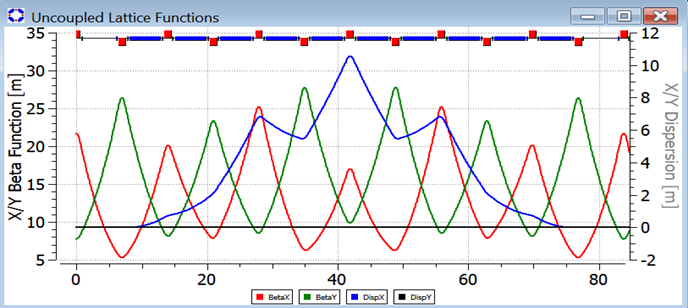
\includegraphics[width=0.8\textwidth]{pring_superperiod}
  \caption{Twiss functions of one superperiod of the electrostatic proton
    ring.}
  \label{fig:pring_superperiod}
\end{figure}

Figure~\ref{fig:pring_twiss} shows the whole ring, which consists of five
superperiods. Each superperiod comprises an achromat with drift spaces at both
ends, so that the phase advance per superperiod is not an integer multiple of
$2\pi$. The ring circumference is \SI{419.1}{m}. The layout of the
electrostatic ring is shown in Fig.~\ref{fig:pring_layout}; it closely
resembles a circle.

\begin{figure}[htbp]
  \centering
  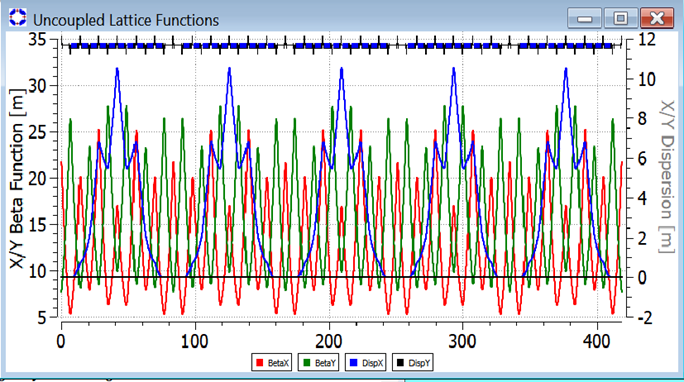
\includegraphics[width=0.8\textwidth]{pring_twiss}
  \caption{Twiss functions along the whole electrostatic proton ring.}
  \label{fig:pring_twiss}
\end{figure}

\begin{figure}[htbp]
  \centering
  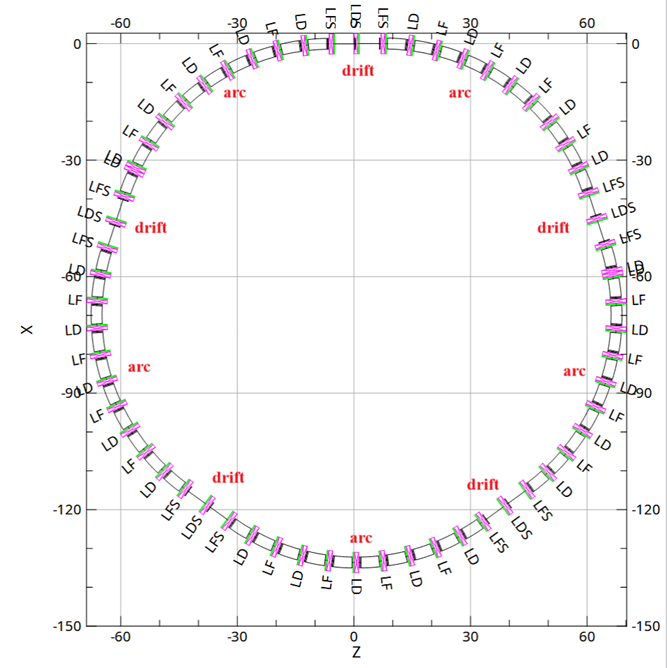
\includegraphics[width=0.6\textwidth]{pring_layout}
  \caption{Layout of the electrostatic proton ring.}
  \label{fig:pring_layout}
\end{figure}

Table~\ref{tab:pring} summarizes the ring parameters required to estimate its
dimensions and cost.

{\small
  \begin{longtable}{p{0.55\textwidth}p{0.38\textwidth}}
    \caption{Parameters of the frozen spin electrostatic ring for the proton
      EDM search.}
    \label{tab:pring} \\
    \toprule
    Parameter & Value \\
    \midrule
    \endfirsthead
    \toprule
    Parameter & Value \\
    \midrule
    \endhead
    Circumference, m & 419.1 \\
    Symmetry order (number of arcs and straight sections) & 5 \\
    Injection energy, MeV & 20 \\
    Proton magnetic anomaly $G$ & 1.793 \\
    Final energy, MeV & 233.8 \\
    EDM experiment energy, MeV & 233.8 \\
    Initial and final relative velocity and Lorentz factor
      & $\beta=0.2$, $\gamma=1.0213$; $\beta=0.6$, $\gamma=1.248$ \\
    Revolution frequency at the beginning and end of the cycle, MHz
      & 0.143--0.429 \\
    Harmonic number & 20 \\
    RF frequency at the beginning and end of the cycle, MHz & 2.8--8.6 \\
    \midrule
    \multicolumn{2}{c}{\textbf{Arcs}} \\
    \midrule
    Arc length, m & 70.1 \\
    Arc superperiodicity & regular lattice \\
    Arc lattice & 5 FODO cells \\
    Number of electrostatic deflectors per arc & 10 \\
    Deflector length, m & 4.39 \\
    Deflector type & cylindrical \\
    Maximum electric field of the deflector, MV/m & 12 \\
    Number of quadrupoles per arc & 9 + 1 (two end halves) \\
    Quadrupole type & electrostatic \\
    Quadrupole families & one focusing (LF), one defocusing (LD) \\
    Maximum quadrupole gradient in the arcs, kV/cm$^2$
      & LF $= 6.78$, LD $= -6.18$ \\
    Quadrupole length, m & 1.0 \\
    Number of chromatic sextupoles per arc & 10 \\
    Sextupole type & electric or magnetic \\
    Sextupole strengths & to be determined \\
    Betatron tunes $\nu_x/\nu_y$ & 6.12/4.72 (preliminary) \\
    Natural chromaticity $\xi_x/\xi_y$ & to be determined \\
    Transition energy, GeV & 3.1 \\
    Maximum $\beta_x/\beta_y$, m & 27.9/34.8 \\
    Maximum horizontal dispersion, m & 10.8 \\
    \midrule
    \multicolumn{2}{c}{\textbf{Straight sections between arcs}} \\
    \midrule
    Length of straight sections, m & $5\times 13.5$ \\
    Lattice of straight sections & DOFFOD \\
    Quadrupole gradients, T/m & QF $= 7.93$, QD $= -7.11$ \\
    Drift length between adjacent quadrupoles, m & 6.0 \\
    \bottomrule
  \end{longtable}
}

As a second option, a racetrack ring with two arcs and dispersion suppressors
at both ends of each arc was considered (Fig.~\ref{fig:pring_suppressor}). One
of the two options will be adopted in the course of further lattice
development, which will take spin decoherence into
account~\cite{Senichev:2013dra}.

\begin{figure}[htbp]
  \centering
  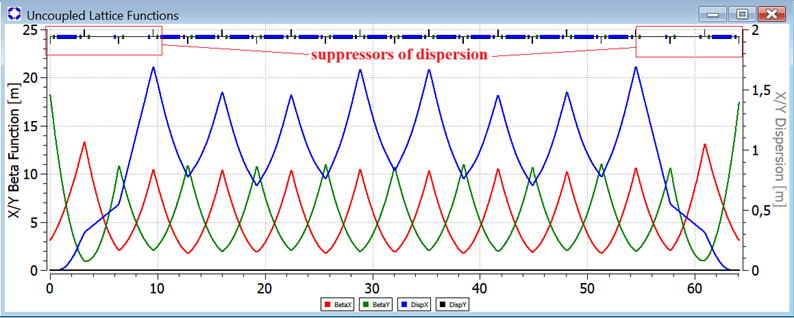
\includegraphics[width=0.9\textwidth]{pring_arc_suppressor}
  \caption{Arc with dispersion suppressors at both ends (racetrack option of
    the proton ring).}
  \label{fig:pring_suppressor}
\end{figure}

\subsection{Frozen spin option for the deuteron beam}

The frozen spin lattice for a deuteron beam differs from the proton one in the
composition of the equipment and in the elements used. Here the bending
deflector with E+B fields consists of electrostatic plates
generating a horizontal electric field, inserted into the gap of a dipole
magnet with a vertical magnetic field (Fig.~\ref{fig:dring_deflector}).

\begin{figure}[htbp]
  \centering
  \begin{panel}[b]{0.38\textwidth}
    \centering
    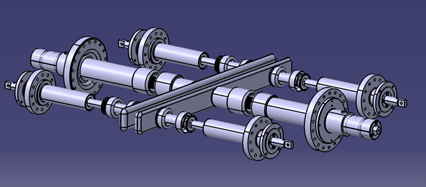
\includegraphics[width=\textwidth]{dring_deflector}
  \end{panel}
  \hfill
  \begin{panel}[b]{0.58\textwidth}
    \centering
    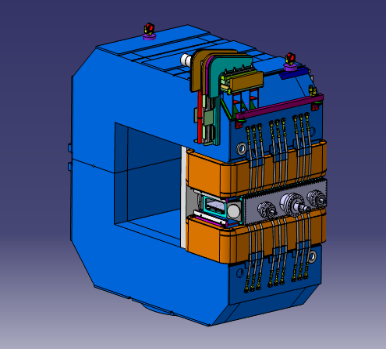
\includegraphics[width=\textwidth]{dring_magnet}
  \end{panel}
  \caption{Electrostatic deflector (a) and vertical-field dipole magnet with
    the electrostatic deflector inserted into its gap (b).}
  \label{fig:dring_deflector}
\end{figure}

The condition of stable motion on an orbit of radius $R$ follows from the
balance of the Lorentz and centrifugal forces:
\begin{equation}
  R = \frac{\gamma m_0 v^2}{e\left|\vec E + c\vec\beta\times\vec B\right|},
  \label{eq:dring_radius}
\end{equation}
from which the momentum precession frequency in the combined fields is
\begin{equation}
  \vec\Omega_p = \frac{e\vec E}{m_0\gamma\beta c} + \frac{e\,c\vec\beta\times\vec B}{m_0\gamma\beta c}.
\end{equation}
Subtracting $\vec\Omega_p$ from $\vec\Omega_{mdm}$ gives the spin precession
frequency relative to the momentum:
\begin{equation}
  \vec\Omega^{p}_{mdm} = \frac{e}{m_0\gamma}\left\{\gamma G\vec B
    + \left(\frac{1}{\gamma^2-1} - G\right)\frac{\vec\beta\times\vec E}{c}\right\}.
\end{equation}

A frozen spin lattice for EDM studies has to satisfy two conditions. The first
relates the external fields to the orbit radius, Eq.~\eqref{eq:dring_radius}
(see also~\cite{Farley:2004hp}). The second requires the spin precession
frequency relative to the direction of motion to vanish,
$\vec\Omega^{p}_{mdm} = 0$, i.e.,
$\gamma G\vec B = -\left(\frac{1}{\gamma^2-1}-G\right)\frac{\vec\beta\times\vec E}{c}$.
This fixes the relation between the fields,
\begin{equation}
  \vec E = -\frac{G\vec B c\gamma^2\beta^2}{\beta\left(1-\gamma^2\beta^2 G\right)},
\end{equation}
and the radius of curvature of the deflector,
\begin{equation}
  R = \frac{\gamma m_0 v^2}{eE\left(1-\dfrac{1}{G\gamma^2}\right)}.
\end{equation}
For an energy of \SI{270}{MeV}, the radius of curvature of the deflector is
$R = \SI{9.207}{m}$, and the total length of all deflectors is
$L_\Sigma = 2\pi R = \SI{57.85}{m}$. With 32 deflectors in total, the length of
a single deflector is $L_{def} = L_\Sigma/32 = \SI{1.808}{m}$.

Figure~\ref{fig:dring_vector} shows the vector diagram that defines the
relative directions of $\vec E$ and $\vec B$. The determining factor is the
positive vertical direction of the magnetic field, which provides the main
compensation of the centrifugal force. Since the deuteron magnetic anomaly is
negative, $G = -0.143$, the axis around which $\vec S$ precesses points
downwards. A zero precession frequency then requires the vector
$\vec\beta\times\vec E$ to point upwards, i.e., the electric field must be
directed as shown in Fig.~\ref{fig:dring_vector}.

\begin{figure}[htbp]
  \centering
  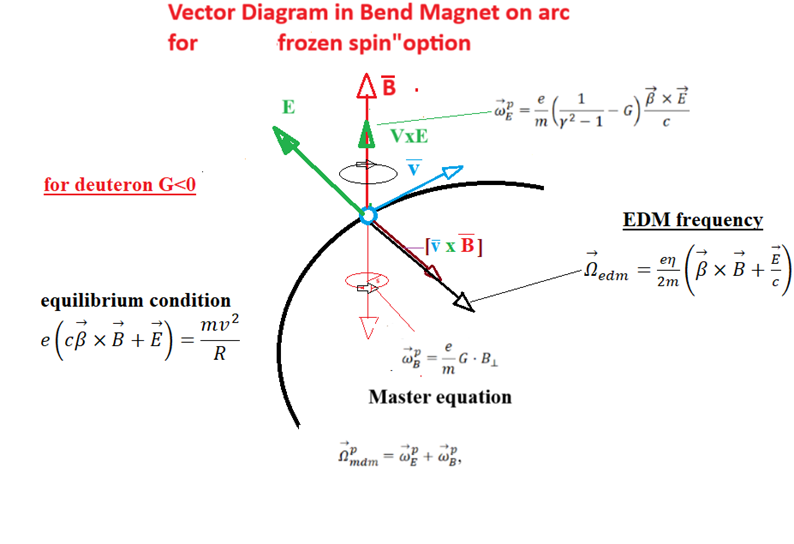
\includegraphics[width=0.75\textwidth]{dring_vector_diagram}
  \caption{Vector diagram of the fields acting on a polarized deuteron.}
  \label{fig:dring_vector}
\end{figure}

Based on these relations, a frozen spin ring lattice was developed.
Figure~\ref{fig:dring_arc} shows the lattice of one arc for the deuteron beam.
The arc consists of two successive achromats with zero dispersion at its middle
and at its ends and comprises eight FODO cells.

\begin{figure}[htbp]
  \centering
  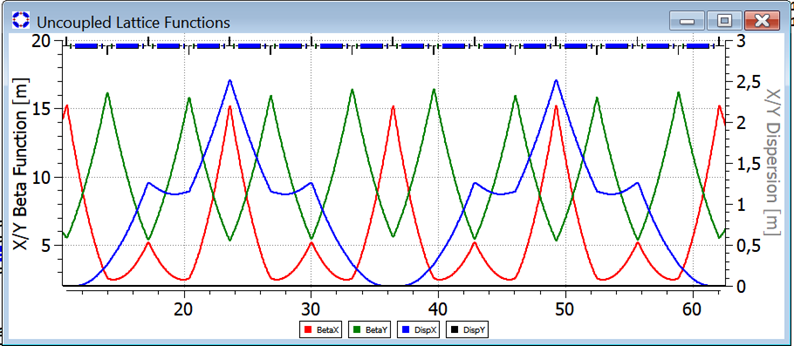
\includegraphics[width=0.85\textwidth]{dring_arc_twiss}
  \caption{Twiss functions along an arc of the frozen spin deuteron ring.}
  \label{fig:dring_arc}
\end{figure}

As in the electrostatic proton ring, the dispersion modulation introduced in
the deuteron lattice provides suitable locations for sextupoles suppressing the
spin chromaticity. Figure~\ref{fig:dring_twiss} shows the Twiss functions of
the whole ring with a circumference of \SI{146}{m}; its layout is shown in
Fig.~\ref{fig:dring_layout}. The main parameters of the synchrotron for the
deuteron EDM search at \SI{270}{MeV} per nucleon are listed in
Table~\ref{tab:dring}.

\begin{figure}[htbp]
  \centering
  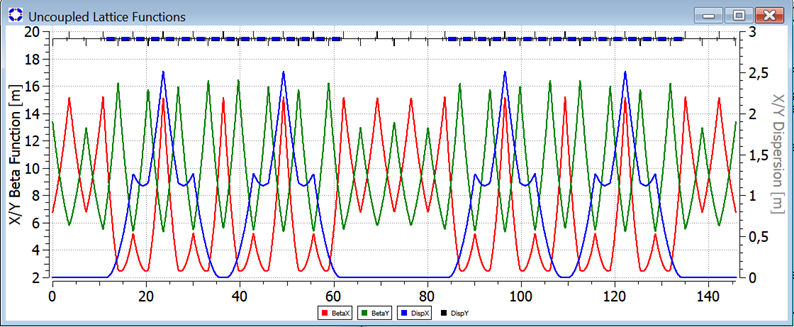
\includegraphics[width=0.85\textwidth]{dring_twiss}
  \caption{Twiss functions along the frozen spin deuteron ring.}
  \label{fig:dring_twiss}
\end{figure}

\begin{figure}[htbp]
  \centering
  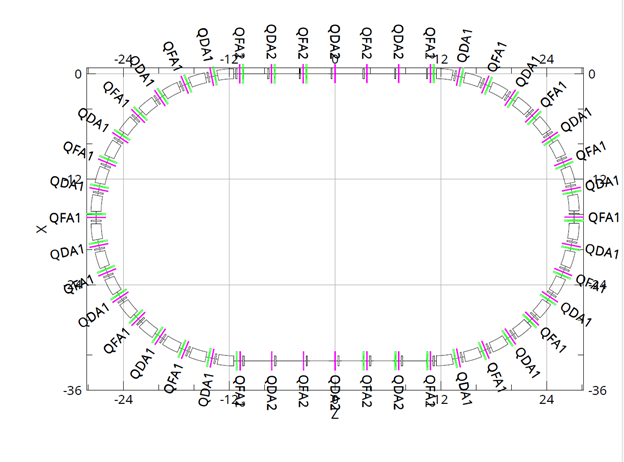
\includegraphics[width=0.6\textwidth]{dring_layout}
  \caption{Layout and dimensions of the frozen spin deuteron ring.}
  \label{fig:dring_layout}
\end{figure}

{\small
  \begin{longtable}{p{0.55\textwidth}p{0.38\textwidth}}
    \caption{Parameters of the frozen spin ring with E+B
      deflectors for the deuteron EDM search.}
    \label{tab:dring} \\
    \toprule
    Parameter & Value \\
    \midrule
    \endfirsthead
    \toprule
    Parameter & Value \\
    \midrule
    \endhead
    Circumference, m & 145.85 \\
    Symmetry order (number of arcs and straight sections) & 2 \\
    Injection energy, MeV/u & 40 \\
    Final energy, MeV/u & 270.0 \\
    EDM experiment energy, MeV/u & 270.0 \\
    Deuteron magnetic anomaly $G$ & $-0.143$ \\
    Initial and final relative velocity and Lorentz factor
      & $\beta=0.2$, $\gamma=1.0213$; $\beta=0.485$, $\gamma=1.143$ \\
    Revolution frequency at the beginning and end of the cycle, MHz
      & 0.143--0.99 \\
    Harmonic number $h$ & 50 \\
    RF frequency at the beginning and end of the cycle, MHz & 7.15--49.9 \\
    Length of the quarter-wave RF cavity, m & 1.502 \\
    Momentum acceptance of the separatrix at maximum energy & $1.31\times10^{-3}$ \\
    Relative momentum spread in the bunch & $5\times10^{-4}$ \\
    \midrule
    \multicolumn{2}{c}{\textbf{Arcs}} \\
    \midrule
    Arc length, m & 51.27 \\
    Arc superperiodicity & 2 \\
    Arc lattice & 4 + 4 FODO cells \\
    Number of E+B deflectors per arc & 16 \\
    Deflector length, m & 1.80 \\
    Deflector type & combined magnetic and electric \\
    Maximum electric field of the deflector, MV/m & 12 \\
    Number of quadrupoles per arc & 15 + 1 (two end halves) \\
    Quadrupole type & magnetic multipole \\
    Quadrupole families & one focusing (QF), one defocusing (QD) \\
    Maximum quadrupole gradient in the arcs, kG/cm
      & QF $= 1.359$, QD $= -1.00$ \\
    Quadrupole length, m & 0.1 \\
    Number of chromatic sextupoles per arc & 16 \\
    Sextupole type & magnetic \\
    Sextupole strengths, kG/cm$^2$ & SF $= 0.12$, SD $= 0.15$ \\
    Betatron tunes $\nu_x/\nu_y$ & 4.70418/2.6140 (preliminary) \\
    Natural chromaticity $\xi_x/\xi_y$ & $-4.91629/{-3.99402}$ \\
    Transition energy, GeV & 5.3 \\
    Maximum $\beta_x/\beta_y$, m & 15.1/16.5 \\
    Maximum horizontal dispersion, m & 2.5 \\
    \midrule
    \multicolumn{2}{c}{\textbf{Straight sections between arcs}} \\
    \midrule
    Length of straight sections, m & $2\times 23.3$ \\
    Lattice of straight sections & $3\times$FODO \\
    Quadrupole gradients, kG/cm & QF $= 0.734$, QD $= -0.782$ \\
    Free drift spaces between adjacent quadrupoles, m & $12\times 3.2$ \\
    \bottomrule
  \end{longtable}
}

\subsection{Summary}

Two specialized frozen spin lattices have been developed for the search for
the proton and deuteron electric dipole moments. These results form the basis
for the physical design of the experimental facilities and their cost
estimate. In contrast to the quasi-frozen spin options of
Sections~\ref{sec:nica-bypass} and~\ref{sec:nuclotron}, these rings are
intended exclusively for experiments on the violation of fundamental
symmetries.

The material of this section has been reported
in~\cite{Palamarchuka:2026pyv,Kolokolchikov:2026xbv}.

\section{Transition energy crossing for polarized protons}
\label{sec:gamma-transition}

\todo[inline]{Draft: this chapter is incomplete and will be extended.}

Collider experiments impose requirements on the luminosity, which, among other
things, limit the longitudinal emittance of the final bunch. During
acceleration, the beam must both cross the transition energy and be split
into 22 bunches by RF gymnastics without blowing up the longitudinal phase
volume.

A possible transition jump scheme for NICA has been considered. Its
characteristic values are the jump amplitude $\Delta\gamma_{tr} = 0.09$ and the
rate of change of the transition energy
$d\gamma_{tr}/dt = \SI{8.5}{s^{-1}}$. With a harmonic RF system, the proposed
jump has little effect on the longitudinal dynamics, since the jump is small
and slow compared with the acceleration rate. With a barrier-bucket RF system,
the jump amplitude is limited by the microwave instability threshold for the
number of particles in a uniform bunch. This limit does not allow reaching
$1\times10^{12}$ particles in the final bunch required for the maximum
luminosity.

The material of this section has been reported
in~\cite{Kolokolchikov:2024hxf,Kolokolchikov:2022akm}.

\section{Spinor technique for spin-orbit tracking}
\label{sec:spinor}

To be written.

\section{Electrostatic elements}
\label{sec:electrostatics}

To be written.

\section{MDM systematics and tensor polarizability}
\label{sec:systematics}

To be written.

\section{Spin precession in the axion search mode}
\label{sec:axion}

Peccei--Quinn axions, proposed as a solution of the strong CP problem, are
among the most likely dark matter candidates. A storage ring can be used as an
antenna for the search for the galactic axion~\cite{Nikolaev:2022wyi}.

Current searches for resonant spin rotation in storage rings use the method
developed by the JEDI collaboration, in which the growth of the vertical
polarization out of the horizontal plane indicates the presence of the axion
field~\cite{Nikolaev:2022wyi}. Based on an analytical treatment of the effect of the spin coherence
time on the frequency scan for the axion signal, an alternative scheme has been
proposed in which an initially vertical spin is rotated into the horizontal
plane~\cite{Nikolaev:2022wyi}. This scheme is free from the ambiguity of the
axion field phase, requires no RF spin flippers, and can be readily
implemented with both deuterons and protons stored in the Nuclotron and NICA
rings.

Consider the proposed experiment on the example of the deuteron EDM search
with polarized beams. It is based on bypasses with Wien filters installed on
them (Section~\ref{sec:nica-bypass}); the QFS lattice of NICA with bypasses is
therefore of particular interest. The EDM and axion experiments differ in that
the axion search does not require the frozen spin condition.

The method relies on the interaction of the axion with the EDM of the particles
in the bunch. This interaction modifies the spin precession described by the
T-BMT equation~\eqref{eq:tbmt} and increases the vertical spin component. Since
the axion mass is unknown, it has to be found by scanning the spin precession
frequency, which is done by varying the fields of the Wien filters.

In the bending arcs of the NICA collider, the particle momentum rotates by
$\Phi^B_{arc} = \pi$, while the deuteron spin ($\gamma G<0$) rotates in the
opposite direction in the horizontal plane relative to the momentum by the
angle $\Phi_s^{arc}$ of Eq.~\eqref{eq:phi_arc} (Fig.~\ref{fig:axion_diagram}).
In each of the two straight sections, the Wien filters rotate the spin back as
described by Eqs.~\eqref{eq:phi_e}--\eqref{eq:wien}. For a maximum electric
field of \SI{120}{kV/cm}, the required magnetic field is below \SI{80}{mT}.

\begin{figure}[htbp]
  \centering
  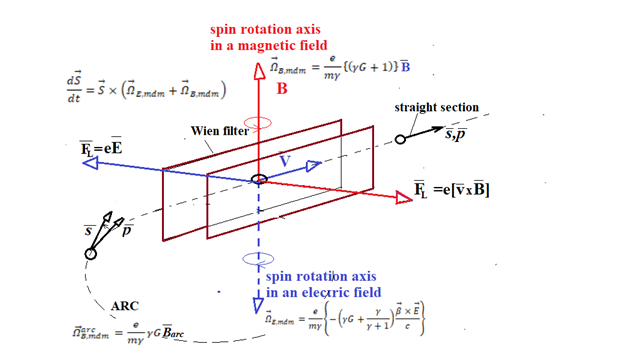
\includegraphics[width=0.75\textwidth]{axion_spin_diagram}
  \caption{Vector diagram of the spin transformation for the deuteron.}
  \label{fig:axion_diagram}
\end{figure}

In the axion search mode, the QFS condition~\eqref{eq:qfs} is modified to
\begin{equation}
  (\gamma G+1)\,\Phi^B_{ss} - \left(\gamma G+\frac{\gamma}{\gamma+1}\right)\beta^2\,\Phi^E_{ss} = \Delta\Phi + \pi\gamma G ,
  \label{eq:axion_qfs}
\end{equation}
where $\Delta\Phi$ is the detuning phase with respect to the QFS case
$\Delta\Phi = 0$. By changing the energy and the Wien filter fields $B_{ss}$
and $E_{ss}$, one changes the frequency of the spin precession around the
vertical axis,
\begin{equation}
  f_{spin} = \frac{\Delta\Phi\,c\beta}{C_{ring}},
  \label{eq:axion_fspin}
\end{equation}
where $C_{ring}$ is the ring circumference, $c\beta$ is the beam velocity and
$\Delta\Phi$ is the detuning phase defined by Eq.~\eqref{eq:axion_qfs}. For
example, at $\Delta\Phi = \SI{1}{rad}$ the spin precession frequency around the
vertical axis is \SI{270}{kHz}, i.e., the axion search range is
$f_{spin} = 0$--\SI{270}{kHz}.\todo[inline]{Eq.~\eqref{eq:axion_fspin} gives an
angular frequency (rad/s); the frequency in Hz is $f_{spin}/2\pi$.}

For a proton beam, the QFS option cannot be realized in NICA: the proton
magnetic anomaly $G_p = 1.793$ is an order of magnitude larger, and the spin
rotates by more than \ang{360} in each arc, so that the accumulated EDM signal
practically vanishes. For the axion search, however, the idea remains valid,
in a different range of $f_{spin}$.

The material of this section has been reported
in~\cite{Nikolaev:2022wyi,Senichev:2022ide,Aksentev:2026mjw}.

\section{Conclusion}
\label{sec:conclusion}

Three lattice options for a storage-ring search for the electric dipole
moments of light nuclei at JINR have been presented.

The NICA collider can be used as a storage ring for EDM experiments by adding
bypass channels parallel to the original straight sections. Wien filters
installed in the bypasses compensate the MDM spin rotation in the arcs, while
the arcs remain unchanged, so that NICA keeps its collider functions. The most
realistic bypass, with a fully regular straight section, satisfies all optical
requirements, and spin-orbit tracking confirms that the quasi-frozen spin
method can be realized in NICA. The simultaneous control of betatron and spin
chromaticity is under study, and the same lattice allows NICA to be used as an
axion antenna.

The Nuclotron can be modernized for deuteron and proton EDM experiments in
the quasi-frozen spin mode with electrostatic deflectors or Wien filters. If
the Nuclotron serves as the collider booster, its final energy can be lowered
to 2--\SI{3}{GeV}, which frees about \SI{70}{m} of the orbit for
polarization-preserving solenoids and EDM and axion equipment.

Finally, two specialized frozen spin rings have been designed: a purely
electrostatic proton ring with a circumference of \SI{419.1}{m} and a
deuteron ring with combined E+B deflectors with a circumference of
\SI{145.85}{m}. These lattices form the basis for the physical design and cost
estimate of facilities intended for the search for the violation of
fundamental symmetries.


\begin{acknowledgments}
This work was supported by the Russian Science Foundation, grant
No.~25-72-30005 (\url{https://rscf.ru/project/25-72-30005/}).
\end{acknowledgments}

\bibliography{bib/references}

\end{document}
